\section{Description of the WHOTS-15 Mooring Cruises}

\subsection{WHOTS-15 Cruise: WHOTS-15 Mooring Deployment}

The Woods Hole Oceanographic Institution Upper Ocean Processes Group (WHOI/UOP), with the UH group's assistance, conducted the fifteenth deployment of the WHOTS mooring onboard the NOAA Ship Hi’ialakai during the WHOTS-15 cruise between September 21st and September 29th, 2018.  The WHOTS-15 mooring was deployed at Station 50 on September 23rd, 2018, 01:17 UTC at 22° 45.94 'N, 157° 53.70 'W, and the WHOTS-14 mooring were recovered on September 27th. The scientific personnel that participated during the cruise are listed in Table II \ref{tab:table_1} 



\begin{table}[hbp]

    \caption{Scientific personnel on Ship Hi’ialakai during the WHOTS-15 deployment cruise}
    
\begin{center}

\begin{tabular}{| l | l | l | l}
   
    \hline
    \textbf{Name} & \textbf{Title} or \textbf{Function} & \textbf{Affiliation} \\
    
    \hline
    Plueddeman, Albert & Chief Scientist & WHOI \\
    \hline
    Pietro, Ben &	Senior Engineering Assistant & WHOI \\
    \hline
    Hasbrouck, Emerson	 & Engineering Assistant & WHOI \\
    \hline
    Greenwood, Ben & Research Associate &	WHOI \\
    \hline
    Snyder, Jefrey & Marine Electronics Technician	& UH \\
    \hline
    Santiago-Mandujano, Fernando & Research Associate & UH \\
    \hline
    Natarov, Svetlana & Research Associate & UH \\
    \hline
    Hebert, Garret & Undergraduate Volunteer  & UH \\
    \hline
    Howins, Noah & Undergraduate Volunteer & UH \\
    \hline
    Maloney, Kelsey & Student Assistant & UH \\
    \hline
    Todd, James & Program Manager & CPO \\
    \hline

\end{tabular}

\end{center}

\label{tab:table_1}

\end{table}


The UH group conducted the shipboard oceanographic observations during the cruise. 

A Sea-Bird CTD (conductivity, temperature, and depth) system was used to measure T, S, and O2 profiles during CTD casts. The time, location, and maximum CTD pressure for each profile are listed in Table II \ref{tab:table_2}. Twelve CTD casts were conducted during the WHOTS-15 cruise. CTD profile data were collected at Station 52 (near the WHOTS-14 buoy) and Station 50 (near the WHOTS-15 buoy). A test cast was conducted at Station 20 (21°29.06’N 158°22.04’W) offshore of Makaha, HI, to an approximate depth of 1500 m to test three acoustic releases. Six CTD yo-yo casts were conducted to obtain profiles for comparison with subsurface instruments on the WHOTS-15 mooring after deployment, and five yo-yo casts were performed for comparison with the WHOTS-14 mooring before recovery. These casts were started less than 0.5 nm from the buoys with varying drift during each cast and consisted of 5 up-down cycles between near the surface and 200 m.


\begin{table}[hbp]

    \caption{CTD stations occupied during the WHOTS-15 cruise }
    
\begin{center}
\begin{tabular}{| c | c | c | c | c | c}
   
    \hline
    \textbf{Station/cast} & 
    \textbf{Date} & 
    \vtop{\hbox{\strut \textbf{Time}}\hbox{\strut \textbf{UTC}}}   & 
    \vtop{\hbox{\strut \textbf{Location}}\hbox{\strut \textbf{(NMEA)}}}   &
    \textbf{Max Pressure (dbar)} \\
    
    \hline 
     20 / 1 & 09/22/2018 & 03:19 & 21° 29.06´ N, 158° 22.04´ W  & 1518\\ 
    
    \hline

\end{tabular}
\end{center}
\label{tab:table_2}
\end{table}










%This is my text. You can see the in Figure \href{fig:banana1}.

\begin{figure}[htbp]
	\begin{center}
		 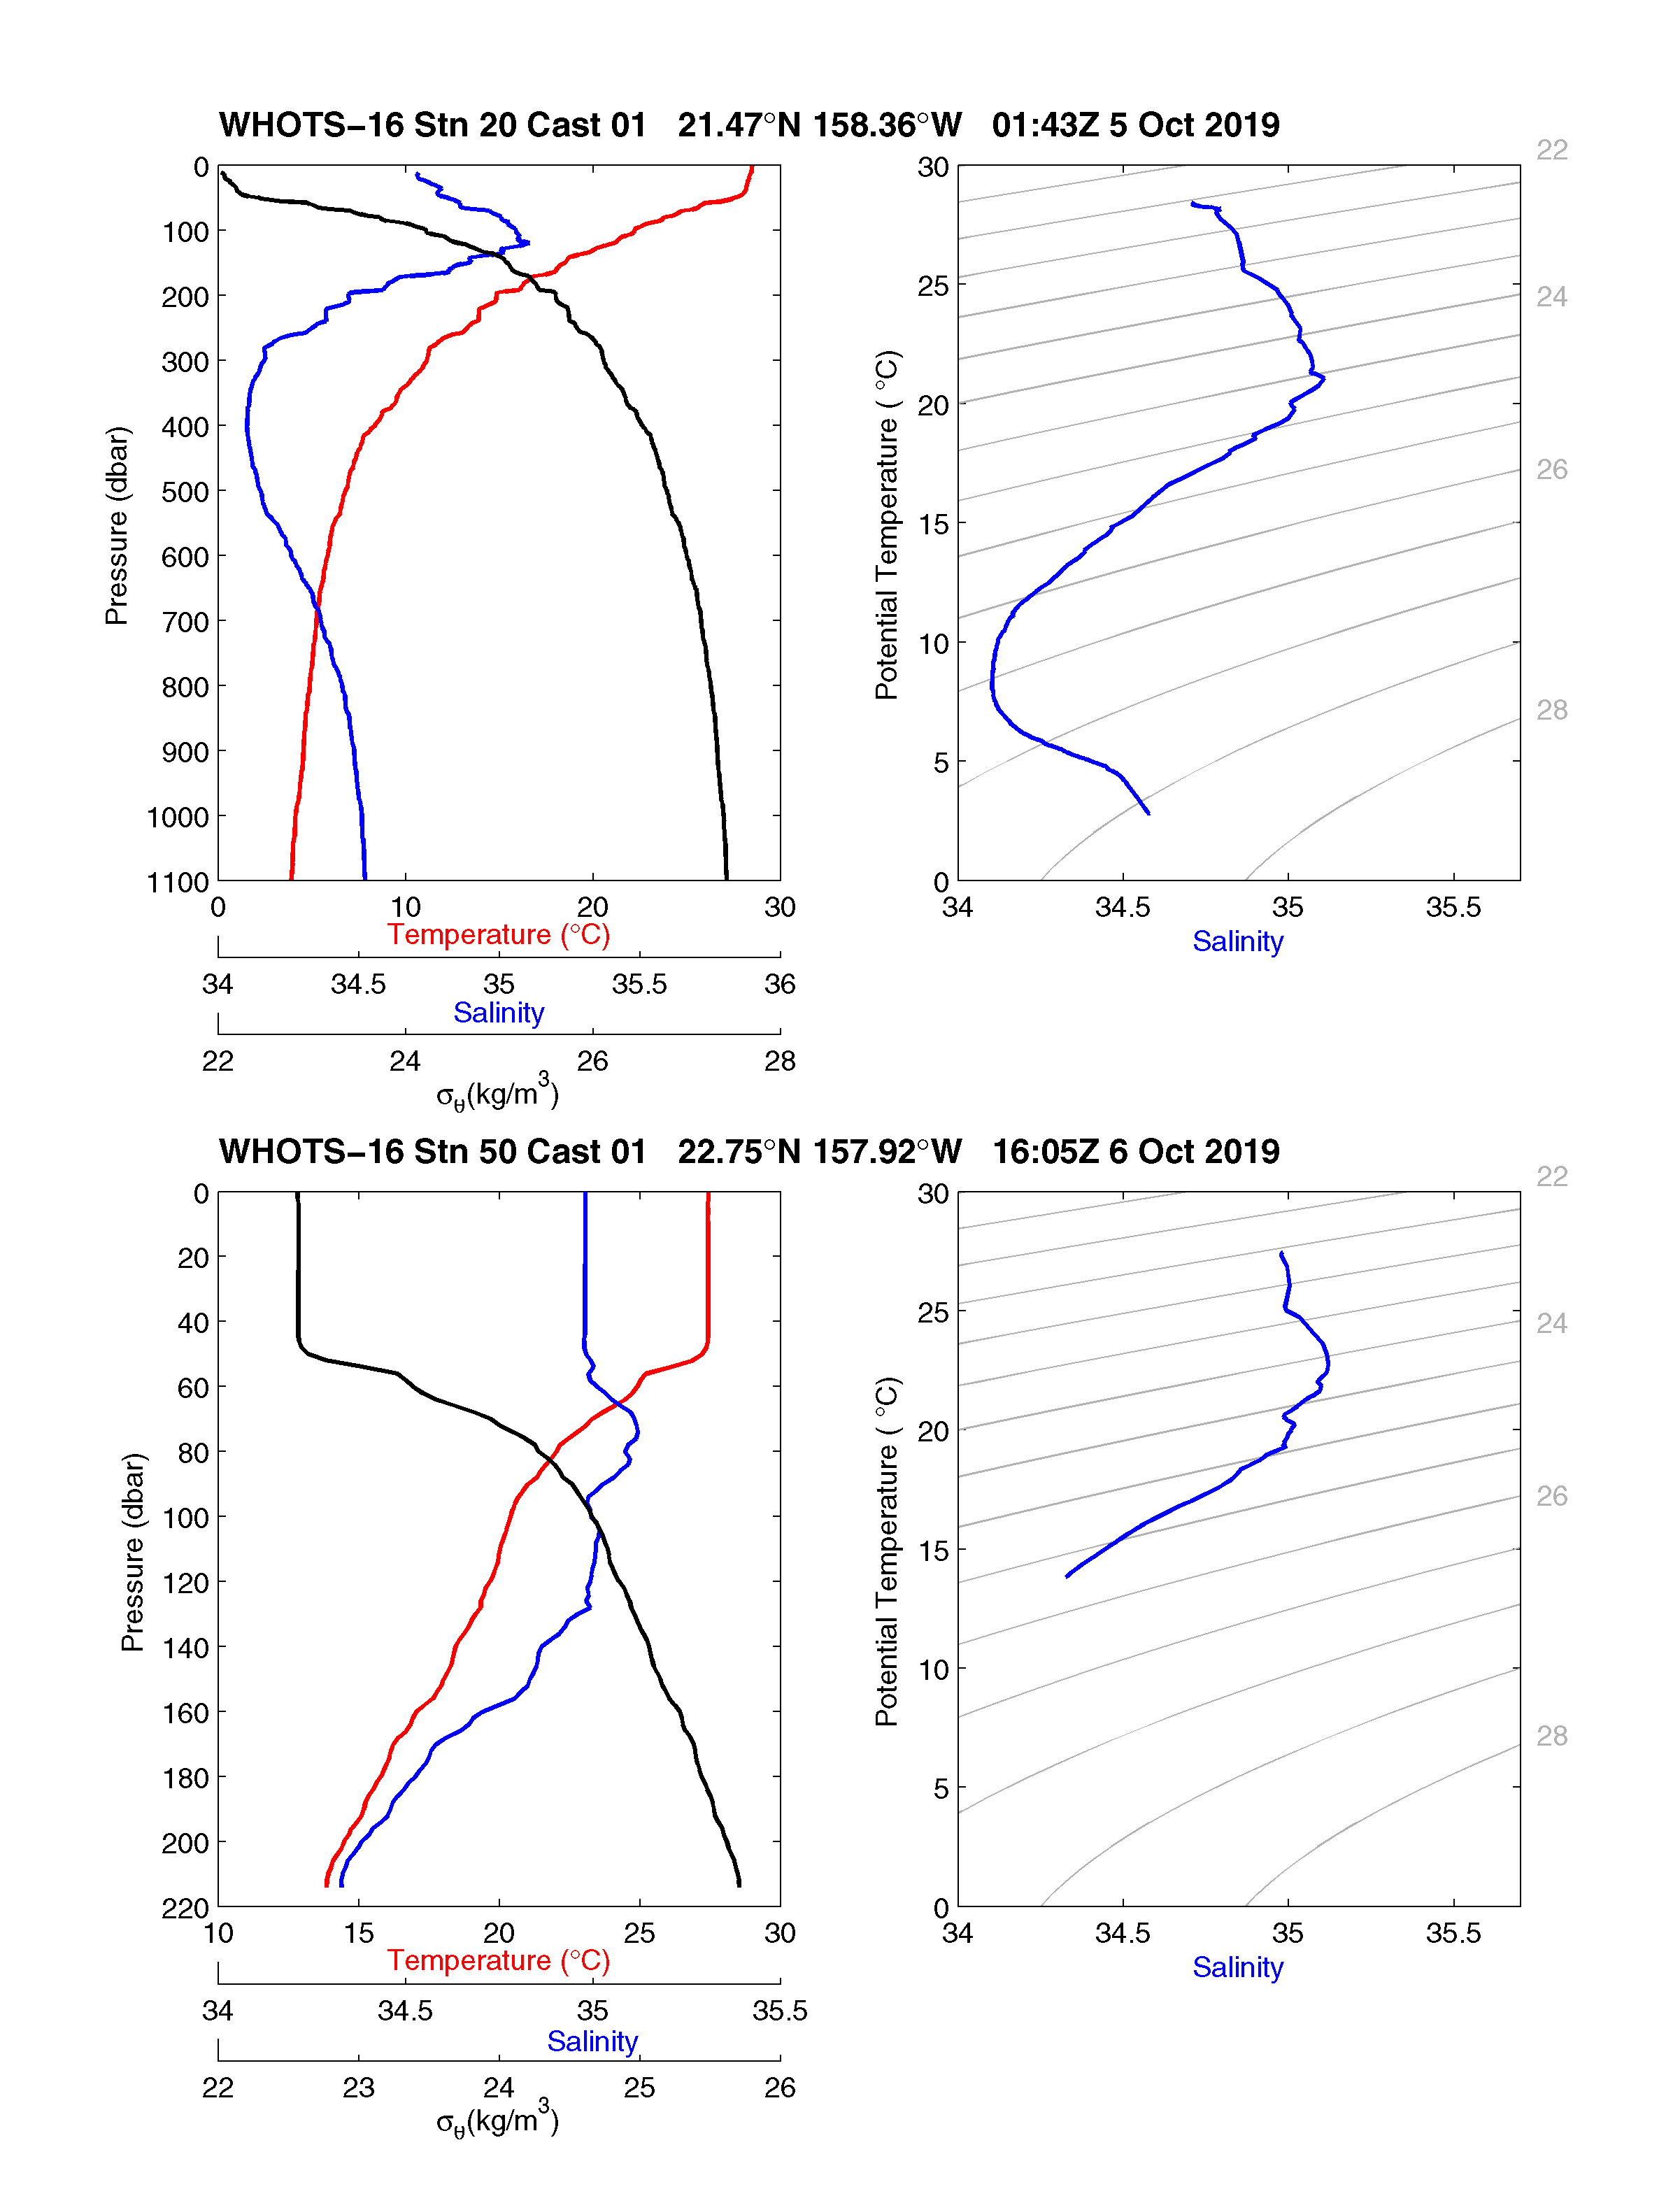
\includegraphics{2.Figures/ctd/2.whots_/s20c1_s50c1.png}
		 \caption{TEST on this one}
		 \label{fig:test1}
	\end{center}
\end{figure}                                      
